\chapter{相关概念及研究}
\label{ch2}

本章首先介绍了 CAV 的网络系统架构,主要从六个方面介绍,包括 TSP 云
服务、V2X 车载通信、车载网络、CAN 总线、IVI、T-BOX,分别分析了它们的
系统架构的组成和原理,最后从云平台、APP、T-BOX、IVI、CAN 总线、ECU、
车间通信七个方面介绍了智能网联汽车所面临的安全威胁

\section{智能网联汽车联网系统架构}

\subsection*{2.1.1 车载网络架构划分}
智能网联汽车是指车联网与智能车的有机联合,是搭载先进的车载传感器、控制器、执行器等装置,并融合现代通信与网络技术,
实现车与人、路、后台等智能信息交换共享,实现安全、舒适、节能、高效行驶,并最终可替代人来操作的新一代汽车\cite{icvsintro}。
车联网在智能辅助驾驶、智能交通规划等领域,都具有不错的应用前景。
车载网络架构如图2.1所示。这是一个
以域为中心的体系结构,具有以太网作为主干,分为五个领域:动力系统、底盘、车
身、信息娱乐和高级驾驶辅助系统(ADAS)。每个域控制
器通过一个中央网关与以太网主干连接。CAN/CAN FD 和
LIN 用作每个域中的通信协议。此外,车载网络可以通
过远程信息处理单元和接口(如 OBD、USB 和 Wi-Fi)连接
到外部网络。这种集中式架构通过域控制器和以太网提
供智能网联汽车所需的计算和通信能力。然而,车辆的外部接
口也增加了。这些开放的接口给智能网联汽车带来了新的攻击
面和安全隐患。为了更好地描述安全威胁,我们提出了
基于这种架构的三层车载网络模型。
\begin{itemize}
    \item 终端节点层: 这一层包含车辆中各个域的 ECU 节点、
    传感器和执行器。这是模型的中心部分。如果受到攻
    击,它会直接影响车辆的安全。
    \item 网络通信层:该层由各种车载网络通信协议组成,如
    以太网、CAN/CAN FD、LIN 等。这一层的主要目的是传
    输数据并与之交互。
    \item 接口设备层:这一层包括各种可以与外部环境交互的通
    信设备接口,如 OBD、USB 等。
\end{itemize}
\begin{figure}
  \centering
  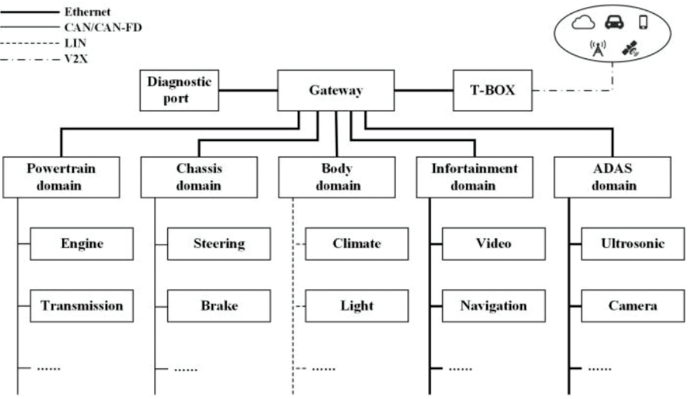
\includegraphics[scale=0.6]{resources/img/i1.png}
  \caption{车联网网络架构图}
\end{figure}
目前的汽车结构中,车辆内部网络主要由 CAN
总线和 ECU 组成。ECU 是嵌入式设备,包括各种智能系统,如无钥匙控制单元
(KCU,key control unit)、防抱死制动系统(ABS,
antilock brake system)、BCM 和紧急制动辅助
(EBA,electronic brake assist)等,通常被用于监控
车辆状态、控制车辆行为。CAN 总线是 ECU 之间
通信的桥梁,负责将汽车内部各 ECU 连接起来,
使它们能够进行高效的信息通信。
\newline
CAN 总线与大量嵌入式设备的多功能连接在为用户提供便利服务的同时,也带来了一些易入侵的接口。恶意攻击者能够利用车载信
息娱乐(IVI,in-vehicle infotainment)系统的 USB
接口和 Wi-Fi 接口恶意窃取用户隐私信息,甚至能
够利用 IVI 系统入侵 CAN 达到控制车辆的目的。
车载诊断(OBD-II,on-board diagnostics-II)接口
是美国工程师协会在 20世纪90年代制定CAN总
线规范时规定开放的车载诊断接口,通常被用来
检测汽车故障并监测汽车尾气排放。然而,OBD-II 接口也很容易成为恶意攻击者非法窃取汽车 CAN 总线数据的入口。此外,T-BOX、胎压
侦测系统(TPMS,tire pressure monitoring system)、RKE、ABS 等大量嵌入式设备都存在可被
利用的攻击面。
这里简单的介绍上述英文名词的定义。
\begin{itemize}
    \item CAN 控制器局域网(Controller Area Network,简称CAN或者CAN bus) 是一种功能丰富的车用总线标准。 
    被设计用于在不需要主机(Host)的情况下,允许网络上的单片机和仪器相互通信。 
    它基于消息传递协议,设计之初在车辆上采用复用通信线缆,以降低铜线使用量,后来也被其他行业所使用。
    \item ADAS 可帮助驾驶员进行驾驶和停车功能。通过安全的人机界面,ADAS 提高了汽车和道路的安全性。ADAS 使用传感器和摄像头等自动化技术来检测附近的障碍物或驾驶员错误,并做出相应的反应。ADAS 可以实现不同级别的自动驾驶,具体取决于车内安装的功能。
    \item OBD是英文On-Board Diagnostics的缩写,中文翻译为“车载自动诊断系统”。这个系统将从发动机的运行状况随时监控汽车是否尾气超标,一旦超标,会马上发出警示。当系统出现故障时,故障(MIL)灯或检查发动机(Check Engine)警告灯亮,
    同时动力总成控制模块(PCM)将故障信息存入存储器,通过一定的程序可以将故障码从PCM中读出。根据故障码的提示,维修人员能迅速准确地确定故障的性质和部位。
    \item ECU(Electronic Control Unit)电子控制器单元,又称为汽车的“行车电脑”,它们的用途就是控制汽车的行驶状态以及实现其各种功能。主要是利用各种传感器、总线的数据采集与交换,来判断车辆状态以及司机的意图并通过执行器来操控汽车。
    \item T-BOX作为无线网关,通过4G远程无线通讯、GPS卫星定位、加速度传感和CAN通讯等功能,为整车提供远程通讯接口,提供包括行车数据采集、行驶轨迹记录、车辆故障监控、车辆远程查询和控制(开闭锁、空调控制、车窗控制、发送机扭矩限制、发动机启停)、驾驶行为分析、4G无线热点分享等服务。
\end{itemize}
\section{TSP 云端通信技术}

(Telematics Service Provider)汽车远程服务提供商,在Telematics产业链居于核心地位,上接汽车、车载设备制造商、网络运营商,下接内容提供商。
 Telematics服务集合了位置服务、Gis服务和通信服务等现代计算机技术,为车主和个人提供强大的服务(导航、娱乐、资讯、安防、SNS、远程保养)。
 \begin{figure}
    \centering
    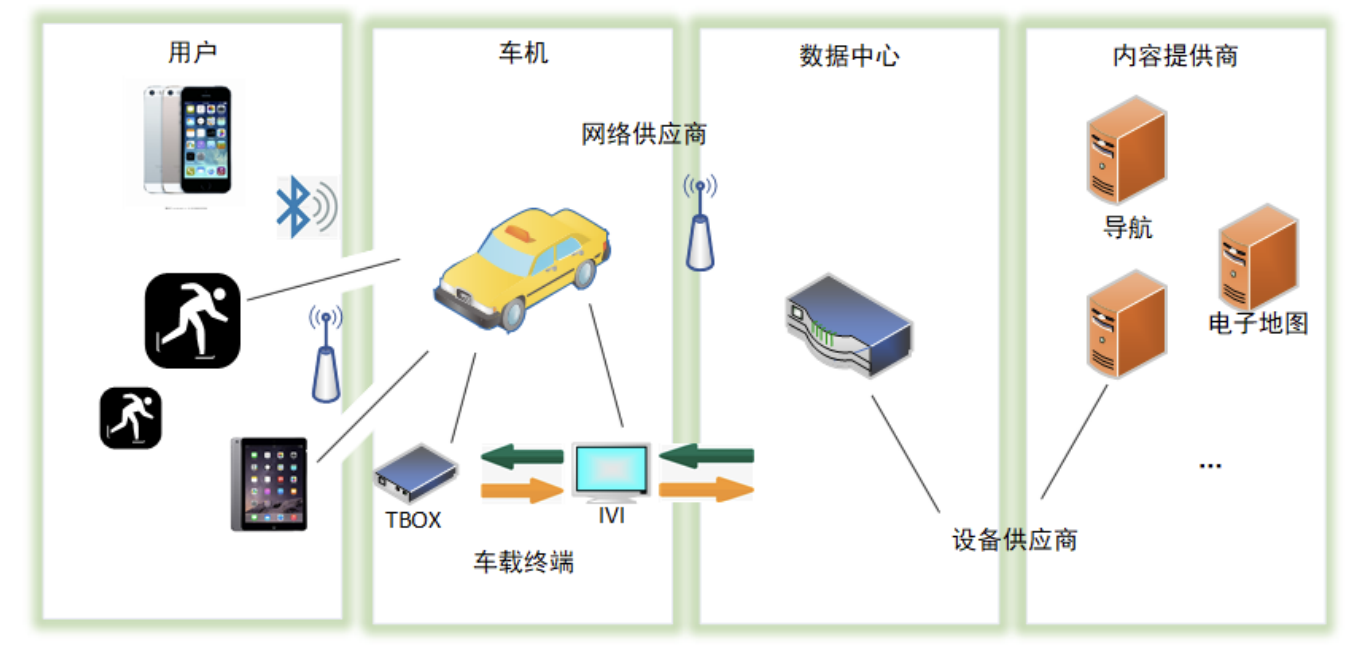
\includegraphics[scale=0.6]{resources/img/i2.png}
    \caption{TSP 系统组成}
  \end{figure}
\newline
通常所说的Telematics就是指应用无线通信技术的车载电脑系统。随着电脑和网络技术应用到汽车上,正在形成称之为Telematics的新的电脑市场。
Telematics是无线通信技术、卫星导航系统、网络通信技术和车载电脑的综合产物,被认为是未来的汽车技术之星。汽车行驶当中出现故障时,通过无线通信连接服务中心,进行远程车辆诊断,
内置在发动机上的计算机记录汽车主要部件的状态,并随时为维修人员提供准确的故障位置和原因。通过终端机接收信息并查看交通地图、路况介绍、交通信息、安全与治安服务以及娱乐信息服务等,
在后座还可以玩电子游戏、网络应用(包括金融、新闻、E-mail等)。通过Telematics提供的服务,用户不仅可以了解交通信息、临近停车场的车位状况,确认当前位置,
还可以与家中的网络服务器连接,及时了解家中的电器运转情况、安全情况以及客人来访情况。也就是说:综合上述所有功能的车载计算机系统叫Telematics。
Telematics系统运作模式就目前发展的模式观察,基本上可将其分为汽车定位系统(GPS)与资讯存取(Access)两部分。
功能特色:卫星定位、道路救援、汽车防窃、自动防撞系统、车况掌握、个人化资讯接收、多媒体娱乐资讯接收。
\newline
Telematics系统的应用领域:基本上可分为前座系统、后座系统与引擎机械系统三大子系统。前座系统主要以安全、车辆保全、驾驶简易性与舒适性为主要考量。后座系统则以多媒体娱乐为主,包括互动式游戏、高传真音响视听系统、随选视讯、数位广播与数位电视等。引擎机械系统,主要是根据车用电脑所收集的车况资讯,进行车况诊断、行车效率最佳化、远距引擎调整或零件预定等。
\newline
Telematics目前主要应用在车载系统上,根据使用目的不同,Telematics可分为三种基本类型,即交通信息与导航服务、安全驾驶与车辆保护及故障诊断的车辆维护服务、娱乐及通信服务。提供全球定位系统技术、地理信息系统、智能型交通系统技术。值得一题的是Telematics逐渐演变为综合了GPS的跟踪装置和无线通信等技术的车载系统。

TSP一词狭义的在互联汽车行业中被用作
对服务提供者进行分类的广义术语
以安全车到云为核心的汽车价值链
数据管理。然而,目前TSP扮演的传统角色
在价值链中不断进化。TSP一词已被
IT公司,系统集成商,甚至一级企业等采用。网络
运营商正在将其M2M/IOT服务扩展到
汽车行业,意图将数据连接“去商品化”。
越来越多的汽车制造商通过TSP创造和集成更多的车载部件。

\section{V2X 车载通信技术}

Vehicle to Everything (V2X) 是一种车载通信系统,支持将信息从车辆传输到可能影响车辆的交通系统的移动部件。V2X 技术的主要目的是提高道路安全、节能和道路交通效率。
\newline
车联网的工作原理: 在 V2X 通信系统中,信息通过高带宽、高可靠性的链路从车辆传感器和其他来源传播,使其能够与其他汽车、停车位和交通信号灯等基础设施以及使用智能手机的行人进行通信。
通过与车辆周围的其他实体共享速度等信息,该技术提高了驾驶员对潜在危险的认识,并有助于降低伤害、道路事故死亡和与其他车辆碰撞的严重程度。
该技术还通过警告驾驶员即将到来的交通、建议替代路线以避免交通和识别可用停车位来提高交通效率。
\newline
V2X 技术的组成部分:
V2X技术的关键组成部分包括V2V(车对车)和V2I(车对基础设施)。V2V 允许车辆与道路上的其他车辆进行通信,而 V2I 允许车辆与外部实体进行通信,例如交通信号灯、停车位、骑自行车的人和行人。这些技术有助于改善道路安全、减少燃料消耗并增强驾驶员与其他道路使用者(例如骑自行车者和行人)之间的体验。

当 V2X 系统集成到传统车辆中时,驾驶员可以接收有关天气模式、附近事故、道路状况、道路工程警告、紧急车辆接近以及使用同一条道路的其他驾驶员活动的重要信息。

配备 V2X 系统的自动驾驶汽车可以为车辆现有的导航系统提供更多信息。该系统还使自动驾驶汽车能够扫描周围环境并根据收到的信息立即做出决定。
\begin{figure}
    \centering
    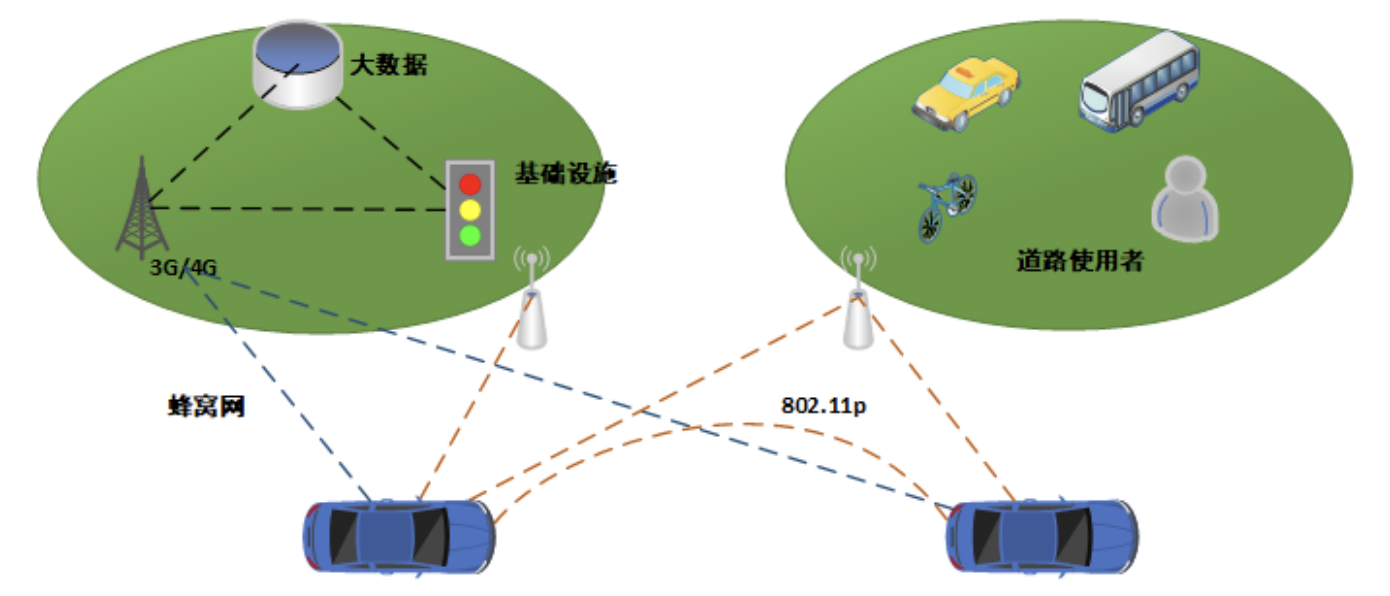
\includegraphics[scale=0.6]{resources/img/i3.png}
    \caption{v2x 应用场景}
  \end{figure}
\newline
如图2.3所示,是基于 V2X 简单的一个应用场景。智能网联汽车不仅可以借
助蜂窝网络,使得汽车与基站、云平台、路边单元等基础设备相连接实现 V2I,
而且还可以通过基站,与周围的车辆进行连接,从而实现 V2V。智能网联汽车在
与其他基础设备、非机动车、车辆、行人等进行通信的时候,使用诸如 802.11p
等协议。

\section{车载内部网络通信技术}
现代车载通信系统中有五种最广泛使用的车载网络:LIN(本地互连网络)、CAN(控制器局域网)、FlexRay、以太网和 MOST(面向媒体的系统传输)。各有优势和劣势。
根据实际观察,LIN 经常用于通常不需要严格时序性能的低速通信。CAN 广泛部署在动力总成和车身控制领域,也是从车辆中检索 OBD(车载诊断)数据的标准接口。
FlexRay 具有高确定性和容错性,
这通常在高级底盘控制和通信主干等应用中需要。有线以太网在量产汽车中仍然相对较新,可能仅用于 ECU 闪烁和有限的网络主干连接等应用。
然而,它在延迟和抖动非常有限的高速数据传输方面具有巨大潜力。因此,以太网在未来可能会获得更多车载网络的份额。

\begin{itemize}
    \item LIN 是一种低成本、低速且易于实现的车载网络,主要用于简单且时间要求不高的应用,例如传统的中央门锁激活、车窗升降器控制、后视镜调节,方向盘按钮模块,以及许多低刷新率传感器。LIN 最突出的优势是它的成本比其他主要网络低得多[18]. 这种优势来自多个方面。首先,LIN控制器相对便宜。LIN 模块使用 UART(通用异步接收器/发送器)端口来发送和接收串行数据。
    \item CAN网络长期以来一直用于传输大部分车载通信信号。尽管后来针对 CAN 无法满足的一些要求开发了各种不同的网络,但 CAN 在汽车网络中仍然保持着普及,特别是在动力总成系统和上半身电子设备中。车辆中的 CAN 芯片估计数量已接近 5 亿个。最近的一项预测甚至预计 CAN 网络将在未来十年内继续在车载通信系统中蓬勃发展。
    \item 出于解决不确定性、增加带宽和增强 LIN 和 CAN 等网络的抗故障能力的目标,FlexRay 由 FlexRay 联盟发起。目前,它已越来越多地应用于车辆动力学领域和域间通信。FlexRay 网络比 LIN 和 CAN 具有更快的传输速度和更高的容错性。它的成本也明显更高,尽管 FlexRay 系统的实际成本可能存在争议。FlexRay 的传输能力有三个最突出的特性: 1) 它可以在同一周期内传输确定性和动态数据;2)它比LIN和CAN(包括TTCAN和CANFD)具有更大的有效载荷;3)在网络拓扑方面非常灵活。
    \item 随着在新型车辆中越来越多地实施 ADAS 和多媒体功能,强烈要求更宽的车辆网络带宽。以太网是超越 CAN 和 FlexRay 的下一代车载网络的一个非常有前途的候选者。近年来,它越来越受到汽车行业的关注。到 2023 年,以太网在新车中的渗透率将高达 40\%。
\end{itemize}

由于现代车载通信系统几乎总是由运行不同通信协议的各种子网组合而成,因此作为不同子网之间接口的汽车网关对于整个车载通信网络至关重要,不容忽视。

通信系统中的汽车网关通常具有三种可能的功能。首先,它可以作为一个协议桥来促进跨不同子网的数据传输。这也是网关最正统的作用。其次,它可以用来“扩展”网络带宽,网关连接到相同协议的其他子网,以避免一个网段过载。第三,网关可以作为防火墙工作,在其中它起到保护作用,以抵御未经授权的外部访问尝试并最大程度地减少不希望的干扰。

网关有两种分类。如果基于路由机制,网关可以分为消息路由或信号路由。如果根据ECU的整体功能,网关可以分为独立的或集成的。

消息路由网关通常根据路由表将入口消息路由到指定的子网,有时甚至不改变传入消息的 ID 或传输周期(例如,路由到相同协议但具有不同协议的网络)波特率)。参考 OSI 模型,只需要到网络层的功能来完成消息路由。相反,信号路由网关需要解包入口消息,重构新消息,并将它们发送到指定的子网。通常,信号路由网关比消息路由网关的计算要求更高,并且可能需要在 OSI 模型方面实现高于网络层的软件。不同协议之间的网关(例如 CAN 和 FlexRay 之间,

另一方面,独立网关是仅用于路由而没有任何其他应用功能(通常除了网络管理和诊断)的网关。集成网关不仅可以路由消息,还可以部分作为具有其他功能的普通 ECU,例如车身控制或插图面板控制。

在车载网络设计中,独立网关和集成网关之间的选择主要取决于 ECU 的成本和计算能力。集成网关更便宜,但需要更多的计算能力,因为它们还需要同时完成非路由任务。独立网关可能会带来额外的硬件成本,例如新的 ECU 和电线,但可以在系统设计、组件测试、维护甚至封装方面带来极大的灵活性和便利性。

在为实际应用设计汽车网络网关时,过程变得更加复杂,并且可能因情况而异。在高度分布式的车载网络中,如何应对网络复杂性不断提高、域间通信量大、时序要求严格、带宽需求增加等挑战,已成为当今汽车网关研究的热门话题。此外,网关的软件架构也非常关键。由于网关在汽车中非常灵活,因此其软件也应该非常易于实施,并满足未来开发的可靠性、可维护性、可重用性和可移植性等质量要求。

\section{本章小结}

本章主要介绍了智能网联汽车的系统架构,首先从整体上给出其车联网系
统的架构介绍,然后对 TSP 云服务、V2X,车载网络通信进行了详细分
析,解释了车载网络通信各个协议之前的区别和优劣。为后文叙述系统架构中存在的攻击入口以及漏洞打下基础。
为后续的智能互联汽车威胁模型的提出提供了前置理论来源。